\documentclass[a4paper, 12pt]{article}

\usepackage[czech]{babel}
\usepackage[utf8]{inputenc}

%for bib overfull hbox
\usepackage{xurl}

%math
\usepackage{amsmath}

%biblatex bibliography
\usepackage{csquotes}
\usepackage[backend = biber, sorting = none, giveninits, style = authoryear, defernumbers = true, uniquename = init]{biblatex}
\DeclareNameAlias{default}{family-given}
%add comma between author and year in citations
\renewcommand*{\nameyeardelim}{\addcomma\space}
%change url: to dostupné z
\DeclareFieldFormat{url}{Dostupné z\space\url{#1}}
%create \citejournal
\DeclareCiteCommand{\citejournal}
  {\usebibmacro{prenote}}
  {\usebibmacro{citeindex}%
    \usebibmacro{journal}}
  {\multicitedelim}
  {\usebibmacro{postnote}}
%get rid of In: before journal title
\renewbibmacro{in:}{}
%change and to ampersand in authors
\AtBeginBibliography{%
  \renewcommand*{\finalnamedelim}{%
    \ifnumgreater{\value{liststop}}{2}{\finalandcomma}{}%
    \addcomma\addspace\&\space}%
}
%change order to author year and keep number cit
% \defbibenvironment{bibliography}
%   {\list
%      {\printtext[labelnumberwidth]{%
%     \printfield{labelnumber}}}
%      {\setlength{\labelwidth}{\labelnumberwidth}%
%       \setlength{\leftmargin}{\labelwidth}%
%       \setlength{\labelsep}{\biblabelsep}%
%       \addtolength{\leftmargin}{\labelsep}%
%       \setlength{\itemsep}{\bibitemsep}%
%       \setlength{\parsep}{\bibparsep}}%
%       \renewcommand*{\makelabel}[1]{\hss##1}}
%   {\endlist}
%   {\item}
%
%add the bib file
\addbibresource{citations.bib}
%for biblatex to work with inputenc
\usepackage[T1]{fontenc}
\usepackage{textcomp}

%bold math
\usepackage{bm}

%graphics
\usepackage{graphicx}

%layout and spacing
\usepackage[lmargin=3.5cm, rmargin=2.5cm, tmargin=2.5cm, bmargin=2.5cm]{geometry}

%lineheight 1.5
\usepackage{setspace}
\onehalfspacing

%paragraph spacing
\usepackage[skip=6pt]{parskip}

%tikz for graphs and math figures
\usepackage{tikz}
\usepackage{etoolbox} % ifthen
\usepackage[outline]{contour} % glow around text
\usetikzlibrary{calc} % for adding up coordinates
\usetikzlibrary{decorations.markings,decorations.pathmorphing}
\usetikzlibrary{angles,quotes} % for pic (angle labels)
\usetikzlibrary{arrows.meta} % for arrow size
\usepackage{xfp} % higher precision (16 digits?)
\usetikzlibrary{angles, quotes}
\usetikzlibrary{shapes.geometric}

%styles for spacetime diagrams
\newcommand{\calI}{\mathscr{I}} %\mathcal
\tikzset{>=latex} % for LaTeX arrow head
\colorlet{myred}{red!85!black}
\colorlet{myblue}{blue!80!black}
\colorlet{mygreen}{green!80!black}
\colorlet{mydarkred}{red!55!black}
\colorlet{mylightred}{red!85!black!12}
\colorlet{myfieldred}{mydarkred!5} % for S' background
\colorlet{mydarkblue}{blue!50!black}
\colorlet{mylightblue}{blue!50!black!30}
\colorlet{mylightblue2}{myblue!10}
\colorlet{mypurple}{blue!40!red!80!black}
\colorlet{mydarkgreen}{green!50!black}
\colorlet{mydarkpurple}{blue!40!red!50!black}
\colorlet{myorange}{orange!40!yellow!95!black}
\colorlet{mydarkorange}{orange!40!yellow!85!black}
\colorlet{mybrown}{brown!20!orange!90!black}
\colorlet{mydarkbrown}{brown!20!orange!55!black}
%\colorlet{mylightbrown}{brown!70!red!70!black!12}
\tikzstyle{world line}=[draw = gray,line width=0.3]
\tikzstyle{world line t}=[draw = gray,line width=0.3]
\tikzstyle{world line'}=[draw = black,line width=0.3]
\tikzstyle{mysmallarr}=[-{Latex[length=3,width=2]},thin]
\tikzstyle{mydashed}=[dash pattern=on 3 off 3]
\tikzstyle{rod}=[mydarkbrown,draw=mydarkbrown,double=mybrown,double distance=2pt,
                 line width=0.2,line cap=round,shorten >=1pt,shorten <=1pt]
\tikzstyle{vector}=[->,line width=1,line cap=round]
\tikzstyle{vector'}=[vector,shorten >=1.2]
\tikzstyle{particle}=[mygreen,line width=0.9]
\tikzstyle{photon}=[-{Latex[length=5,width=4]},black,line width=0.8,decorate,
                    decoration={snake,amplitude=1.0,segment length=5,post length=5}]

\def\tick#1#2{\draw[thick] (#1) ++ (#2:0.06) --++ (#2-180:0.12)}
\def\tickp#1#2{\draw[thick,mydarkred] (#1) ++ (#2:0.06) --++ (#2-180:0.12)}
\def\Nsamples{100}

%new section new page
\AddToHook{cmd/section/before}{\clearpage}


\title{Superdeterminismus}
\author{Kryštof Pšenička}




\begin{document}

\maketitle
\tableofcontents
\clearpage
\section{Úvod}
(Zpracováno podle knihy \cite{quantum})

Na konci 19. století se vědci domnívali, že s výjimkou několika detailů jejich teorie dokázaly odpovědět na všechny otázky fyziky. Podle nich už na obzoru nebyly žádné velké objevy. Maxwellovy rovnice elektromagnetismu a Newtonovy pohybové zákony kreslily deterministický vesmír, v němž má každá částice určitou pozici a momentum v daném okamžiku. Síly které působí na částici určují, jak se její pozice a rychlost mění v čase.

Ale už v roce 1900, při řešení problému absolutně černého tělesa, objevil Max Planck kvanta - nedělitelné balíky světla, jejichž velikost (energie) závisí na frekvenci daného světla. I když si v té době Max Planck i většina ostatních fyziků myslela, že to je pouze matematický trik, který nemá žádné implikace ve fyzickém světě, byl to první krok vedoucí ke kvantové revoluci.

Albert Einstein věřil ve fyzickou existenci Planckových kvant a ve vlnově-korpusku\-lární dualitu světla, podle níž je světlo částicí a vlnou zároveň a chová se jako jedno nebo druhé podle způsobu našeho pozorování. Ve svém Annus mirabilis\footnote[1]{Zázračný rok, ve kterém Einstein vydal 4 revoluční vědecké články.} (1905) kvantově vysvětlil fotoefekt: když elektron získá dostatek energie absorbcí kvanta světla, je uvolněn z obalu atomu a následně může být vyzařován.

Francouzský aristokrat Luis de Broglie vzal tento závěr z Planckovy práce ještě dál a teoretizoval o vlnově-korpuskulární dualitě všech částic, nejen světelných, ale také částic hmotných.

Kvantový model atomu se postupně vyvíjel od modelu Nielse Bohra s jedním kvantovým číslem, vyjadřujícím velikost oběžné dráhy elektronu. Arnold Sommerfeld postupně k tomuto modelu přidal 3 další kvantová čísla: jedno vyjadřující tvar eliptické oběžné dráhy elektronu, druhé (magnetické) vyjadřující orientaci oběžné dráhy v prostoru a poslední vyjadřující spin, což je vnitřní moment hybnosti částice.

V této době bylo zřejmé, že je potřeba vytvořit teorii, která by popisovala fenomény kvantového světa: kvantovou mechaniku.

Roku 1925 Werner Heisenberg přišel na Maticovou kvantovou mechaniku. Maticová, protože ve výpočtech využívá matic a vektorů. Matice jsou tabulky čísel (viz Obrázek \ref{fig:1}), které v této teorii mohou vyjadřovat veličiny jako polohu a hybnost částice. Vektory jsou veličiny, které mají kromě velikosti i směr a dají se vyjádřit maticemi. V Maticové mechanice se používají k vyjádření stavu systému. Vzhledem k používaným matematickým prostředkům je tato teorie nesmírně nepraktická k výpočtu vývoje jakéhokoli systému, jelikož rozměry matic se zvyšují exponenciálně s rostoucím počtem částic v systému.

\begin{figure}[ht]
    \centering
    $\begin{pmatrix}
    1 & 0 & 1 \\
    0 & 1 & 0 \\
    1 & 0 & 1
    \end{pmatrix}
    $
    \caption{\label{fig:1}Matice o 3 řádcích a 3 sloupcích.}
\end{figure}

Pouze tři měsíce po vydání Heisenbergova článku o Maticové mechanice zkonstruoval rakouský fyzik Erwin Schrödinger svou proslulou vlnovou rovnici (Rovnice (\ref{eq:1})), která popisuje vývoj vlnové funkce a stala se základem Schrödingerovy vlnové mechaniky. Vlnová mechanika se rychle stala oblíbenější než Maticová, jelikož výpočty s vlnovou rovnicí jsou daleko jednodušší.

\begin{equation}
    \bm{i\hbar \frac{\partial \Psi}{\partial t} = -\frac{\hbar^2}{2m}
    \frac{\partial^2 \Psi}{\partial x^2} + V \Psi}
    \label{eq:1}
\end{equation}

O rok později Schrödinger dokázal matematickou ekvivalenci Maticové a Vlnové mechaniky. Jsou to dvě formy téže teorie - Kvantové mechaniky.

Ve stejném roce Max Born předložil pravděpodobnostní interpretaci vlnové funkce, ve které druhá mocnina vlnové funkce vyjadřuje pravděpodobnostní distribuční funkci výsledku. Pro ilustraci vezměte v úvahu obrázek \ref{fig:2}. $\bm{\Psi}$ je vlnová funkce, která vyjadřuje stav systému, např. pozici elektronu. \textbf{P} je pravděpodobnostní distribuční funkce. Tato funkce vyjadřuje pravděpodobnost pro každý možný výsledek měření (každá možná pozice elektronu). $\bm{P(x_0,x_1)}$ je pravděpodobnost, že výsledek měření bude mezi $x_0$ a $x_1$. V našem případě je to pravděpodobnost, že elektron bude mít pozici mezi $x_0$ a $x_1$ a počítá se integrací pravděpodobnost\-ní funkce mezi hodnotami $x_0$ a $x_1$. Integrací $(\int_{x_0}^{x_1}|\Psi|^2\,dx)$ získáme obsah pod křivkou v daném rozsahu, který odpovídá hledané pravděpodobnosti. 


\clearpage

\begin{figure}[ht]
\centering
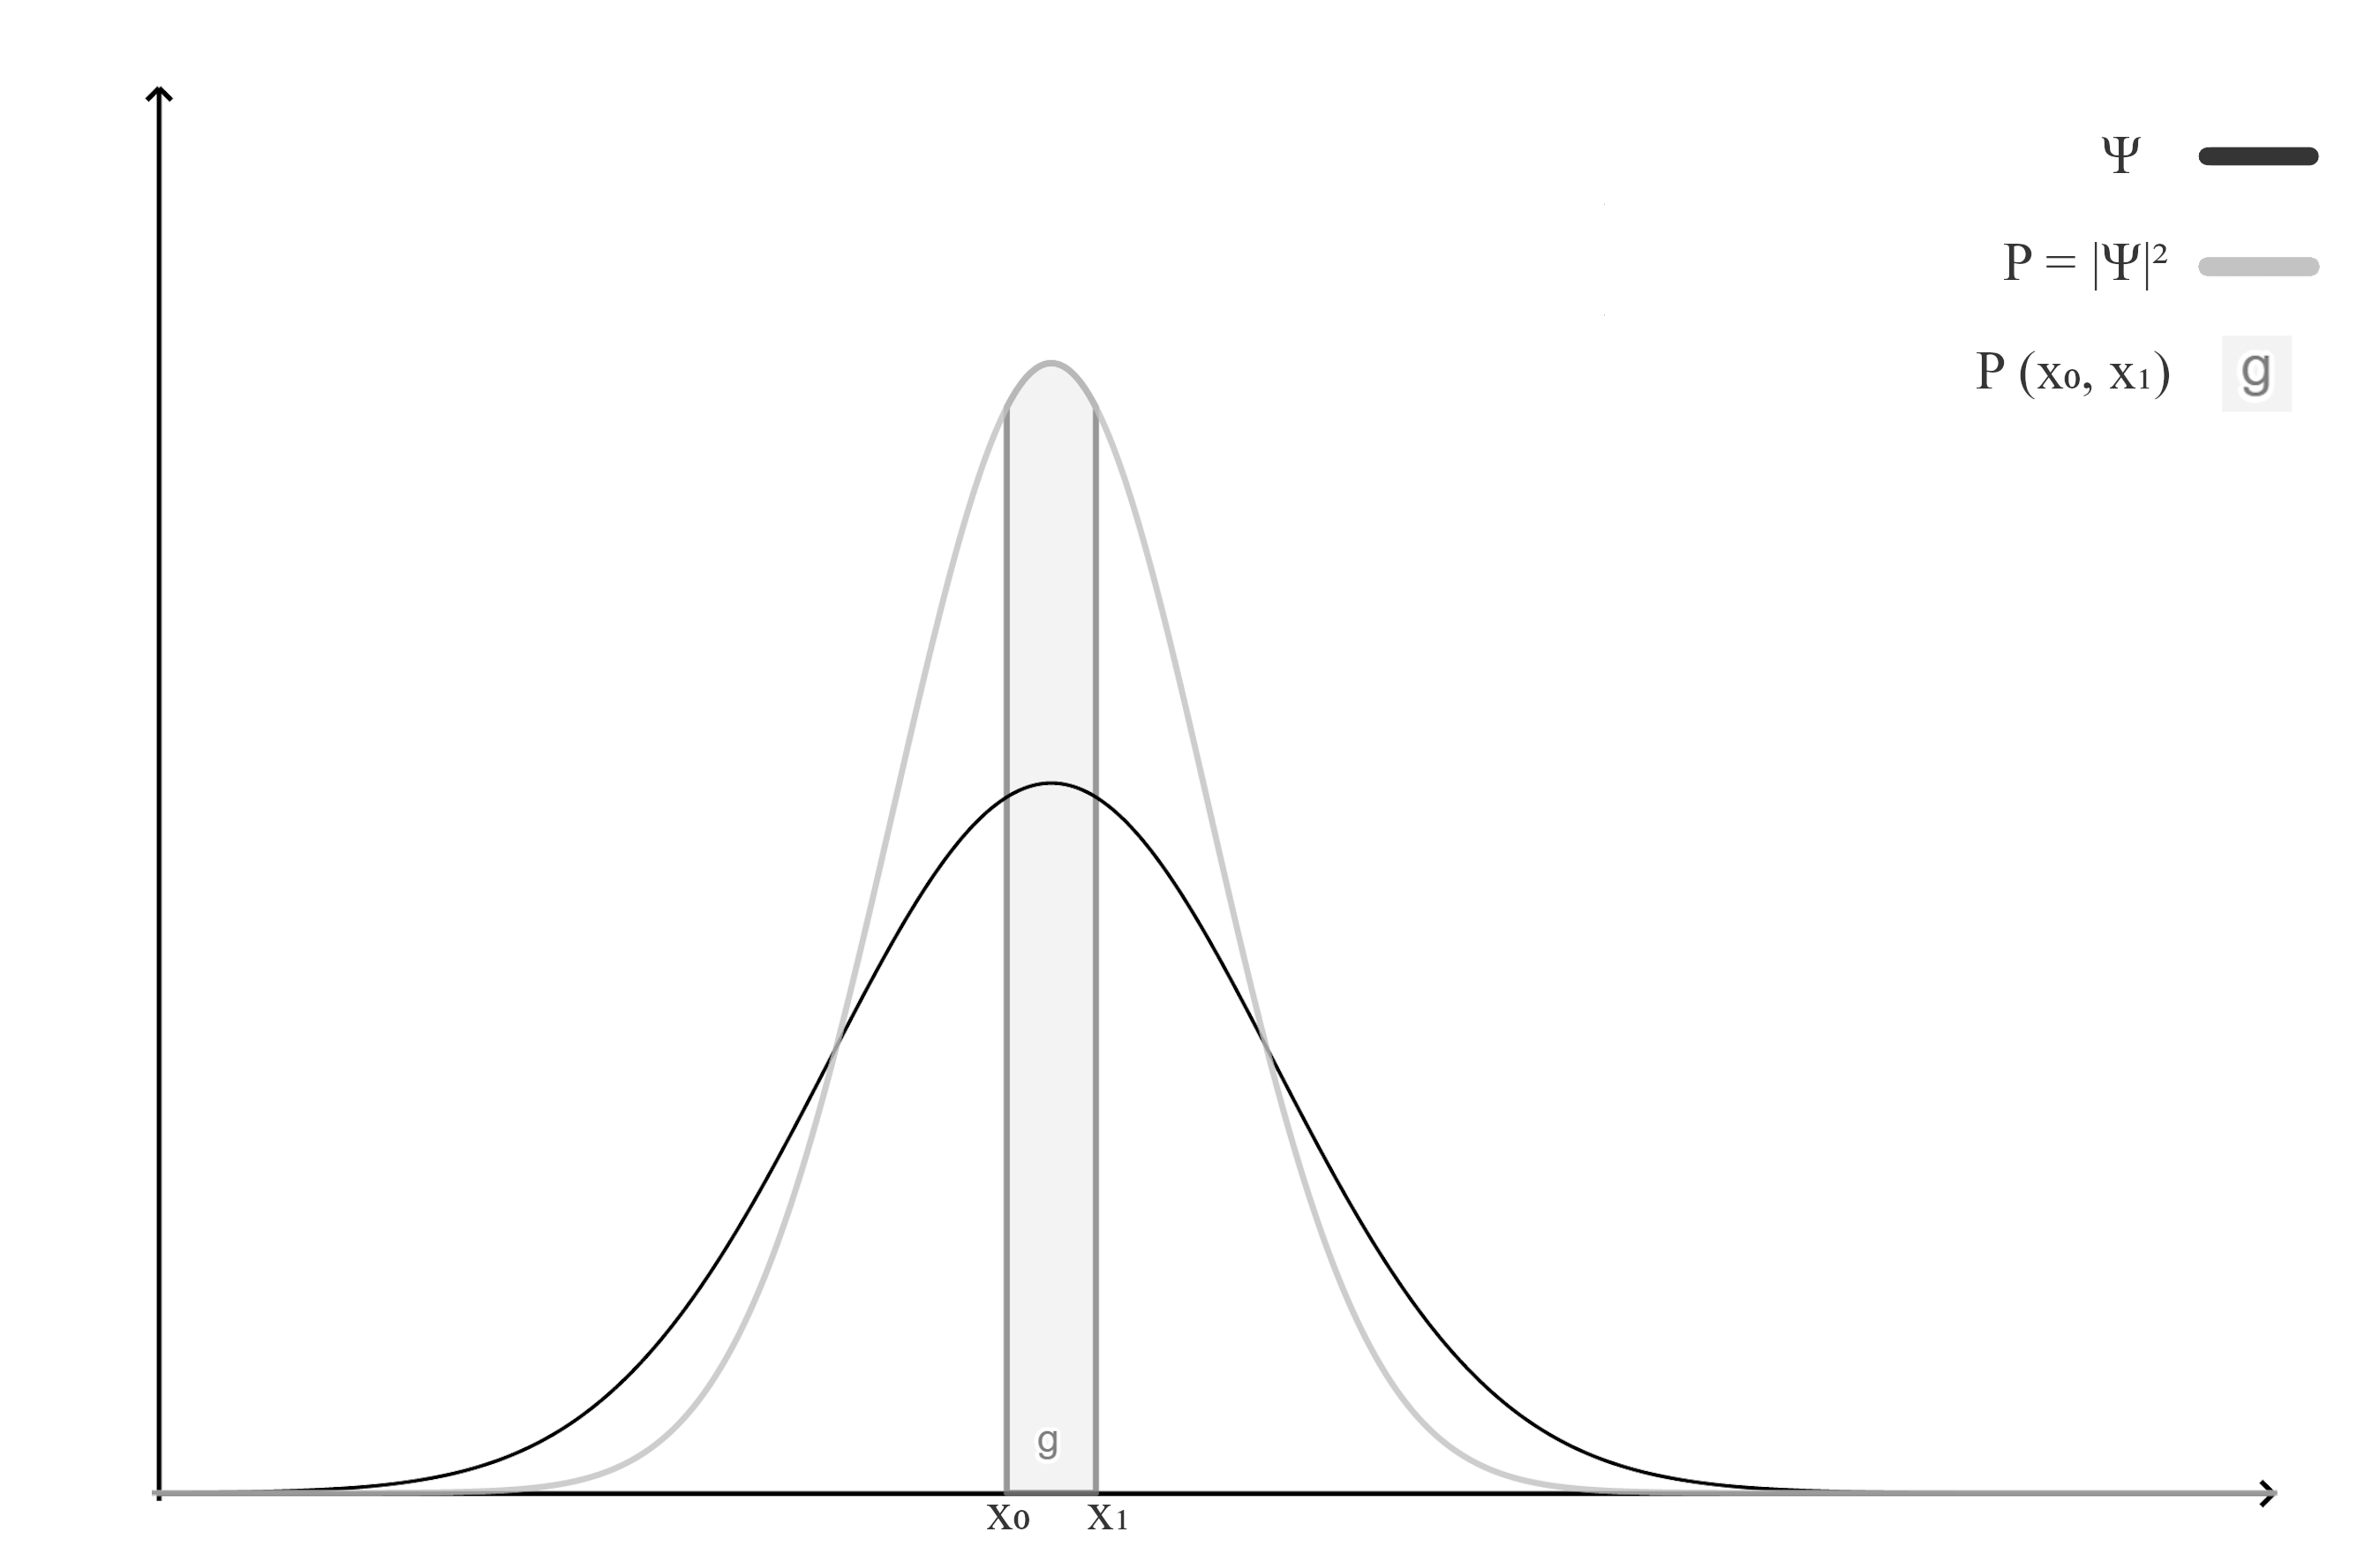
\includegraphics[width=300pt]{images/probability-function.png}
\caption{\label{fig:2}Vlnová funkce, pravděpodobnostní funkce a pravděpodobnost určitého výsledku.}
\end{figure}



Tato pravděpodobnostní interpretace se stala důležitou součástí dnešní Kvantové mechaniky, za kterou je považována Kodaňská interpretace, kterou společně vyhotovili Bohr, Pauli a Heisenberg v Bohrově institutu v Kodani.

Kvantová mechanika změnila obraz vesmíru z deterministického a předurčeného na indeterministický a pravděpodobnostní. V kvantovém pravděpodobnostním vesmíru můžeme určit pouze pravděpodobnost daného výsledku. Jediný způsob, jak Clerk Maxwell a Ludwig Boltzmann mohli popsat vlastnosti plynu skládajícího se z nesčetného množství částic bylo, použitím pravděpodob\-nosti a museli se spokojit se statistickým popisem. Tento nucený ústup ke statistické analýze byl způsoben neuskutečnitelností sledování pozice a rychlosti tolika částic. Pravděpodob\-nost byla důsledkem lidské nevědomosti. Naopak podle Kvantové mechaniky toto pravděpodobnost\-ní vyjádření kvantového světa není způsobeno lidskou nevědomostí, ale je fundamentální vlastností kvantového vesmíru.

Přes jeho účast v začátcích kvantové revoluce se Albert Einstein stal jejím největším kritikem. Uvědomoval si její užitečnost v atomových měřítcích, ale myslel si, že \uv{Bůh ne{hraje v }kostky.} Byl přesvědčený, že kvantová mechanika není konečnou teoríí, že za ní musí být fundamentálnější deterministická teorie. Takovým teoriím se říká teorie se \uv{skrytými} parametry. Podle těchto teorií dokážeme určit jen pravděpodobnost výsledků, jelikož neznáme všechny parametry. Kdybychom znali tyto \uv{skryté} parametry, dokázali bychom určit přesný výsledek měření.

V roce 1962 našel John Stewart Bell způsob, jak matematicky posoudit možnost teorie se skrytými parametry, která by replikovala výsledky kvantové mechaniky. Dnes se jí říká Bellova nerovnost. Tato nerovnost byla experimentálně porušena. Podle všeobecného mínění znamená porušení této nerovnosti nemožnost teorie se skrytými parametry. Toto porušení ale pouze znamená, že neexistuje teorie se skrytými parametry, která splňuje princip lokálního realismu a podmínku Statistické Nezávislosti.

V této práci se budu věnovat teorii se skrytými parametry, která nesplňuje podmínku Statistické Nezávislosti. Takovou teorii nazval Bell Superdeterminismus. Statistická Nezávislost (viz Rovnice (\ref{eq:2})) znamená, že pravděpodobnostní distribuce skrytých parametrů ($\bm{P(\lambda)}$) se nezmění, když vezmeme v potaz nastavení detektorů, \textbf{(a,b)}. Této podmínce se často říká podmín\-ka svobodné vůle, nebo svobodné volby. 

Cílem této práce je přehodnocení argumentů proti Superdeterminismu. Pokusím se vysvětlit, v rozporu s všeobecným míněním, že Superdeterminismus je cestou, která by mohla vyřešit mnoho problémů se současnými teoriemi a kterou bychom neměli ignorovat; je to cesta kterou jsme se nevydali.

\begin{equation}
    \bm{P(\lambda|\bm{a},\bm{b}) = P(\lambda)} 
    \label{eq:2}
\end{equation}



\input{partials/Problemy\_kvant\_mech.tex}
\input{partials/Bellova\_nerovnost.tex}
\section{Superdeterminismus}
\subsection{Definující vlastnosti}
(Zpracováno podle článku \cite{supdet:rethink})

Superdeterministické teorie jsou Psi-epistemické, deterministické a lokální teorie skrytých proměnných, které porušují Statistickou Nezávislost a nemusí být nutně realistické.

\subsubsection{Psi-epistemická}
Podle Psi-epistemické teorie vlnová funkce Schrödingerovy rovnice (Psi, $|\psi\rangle$) neodpovídá přímo vlastnosti nějakého systému v reálném světě. Kodaňská interpretace Kvantové mechaniky je Psi-epistemická, protože považuje vlnovou funkci pouze za reprezentaci znalostí o stavu systému.

Opakem je Psi-ontická teorie, která bere vlnovou funkci jako fundamentální část reálného světa.

Superdeterministické teorie jsou Psi-epistemické v tom smyslu, že vlnová funkce je průměrná pravděpodobnostní reprezentace přesných veličin systému, popsaných hlubší teorií.

Vlnová funkce odvozená ze superdeterministické teorie by se měla řídit dosud ověřenými evolučními zákony kvantové mechaniky. Smysl hledání takové teorie je tedy vytváření předpovědí nad rámec kvantové mechaniky.

\subsubsection{Deterministická}
Roku 1814 formuloval matematik Pierre-Simon de Laplace myšlenku deterministického vesmíru pomocí Laplaceova démona \parencite{laplace:demon}. Podle determinismu by bytost (démon) znající pozici a momentum každé částice ve vesmíru a mající dostatečnou výpočetní sílu mohla pomocí základních zákonů přírody vypočítat minulost i budoucnost každé částice. Vše je předurčené, evoluce každé částice je dána přírodními zákony.

Determinismem myslíme, že evoluční zákon teorie jednoznačně mapuje stavy systému v čase \textbf{\emph{t}} na stavy v čase \textbf{\emph{t'}} pro libovolné \textbf{\emph{t}} a \textbf{\emph{t'}}.

Jelikož Kvantová mechanika není deterministická, musí deterministická teorie reprodukující Kvantovou mechaniku obsahovat skryté proměnné. Skryté proměnné, nadále kolektivně označované $\bm{\lambda}$, obsahují všechny informace potřebné k určení výsledku měření kromě \uv{neskrytých} proměnných, které jsou obsaženy v přípravě stavu systému.

Je důležité poznamenat, že tyto skryté proměnné nemusí být vlastní pro měřený systém, ani v něm lokalizované. Představme si chlapce jménem Nikolaj, který má na mysli dvě otázky: \uv{Jaká je moje hmotnost?} a \uv{Zvládnu úspěšně udělat maturitní zkoušky?} V deterministickém vesmíru se odpovědi na obě otázky nacházejí v současném stavu vesmíru, ale jejich dostupnost je velmi odlišná. Informace o hmotnosti Nikolaje se vyskytuje lokálně v něm samotném, zatímco informace o jeho úspěšnosti při maturitní zkoušce je rozložena po většině prostoru současné chvíle.

\subsubsection{Lokální}
(Zpracováno podle článku \cite{CoA})

Lokalitou v Superdeterminismu exkluzivně myslíme Kontinuitu Působení (dále jen KoP). Zvažme oddělené časoprostorové oblasti $\bm{1}$ a $\bm{2}$ (viz Obrázek \ref{fig:7}), přičemž $\bm{1}$ je obklopena \uv{zastiňovací} oblastí $\bm{S}$. $\bm{S}$ není pouze prostorovou oblastí, zahrnuje budoucnost i minulost oblasti $\bm{1}$ a zároveň i její prostorový rozsah (v dimenzích $\bm{x,y,z}$).

\begin{figure}[ht]

    \centering

    \begin{tikzpicture}[scale=0.85]
        % S
        \draw (2, 4) circle (1.3);
        \draw (2, 4) circle (1);

        \draw[<-] (3.15, 4) -- (4, 3) node[below] (S) {$S$};
        
        %1
        \draw (2, 4) node  (1) {$1$};
        \draw (2, 4) circle (0.5);
        
        %2
        \draw (5.5, 3) node  (2) {$2$};
        \draw (5.5, 3) circle (0.5);
        
        
        % Axes
        \draw[->] (0, 0) -- (7,0) node[below] (x,y,z) {$x,y,z$};
        \draw[->] (0, 0) -- (0,7) node[left] (t) {$t$};
    \end{tikzpicture}
    \caption{\label{fig:7}Kontinuita Působení zobrazená v časoprostorovém diagramu. $t$ je časová osa a $x,y,z$ je prostorová osa, znázorňující všechny 3 prostorové dimenze.}
\end{figure}

Matematický model porušuje KoP, pokud dovoluje \uv{působení na dálku}, tzn. pokud změny ve $\bm{2}$ souvisejí se změnami v $\bm{1}$, aniž by souvisely se změnami uvnitř $\bm{S}$. $\bm{S}$ je jakási kontrolovací oblast pro KoP. Jestliže se nějaká informace dostane z $\bm{1}$ do $\bm{2}$, musí se také nacházet v $\bm{S}$, aby model dodržoval KoP. Jako příklad můžeme uvést systém kohoutku, trubek a fontány. Aby model s kohoutkem ve $\bm{2}$ a korelovanou fontánou v $\bm{1}$ splňoval KoP, musí obsahovat popis zprostředkujících parametrů (Např. tok vody trubkami mezi kohoutkem a fontánou) v přechodné zastiňovací oblasti $\bm{S}$. V takovém modelu jsou při znalosti všech parametrů v $\bm{S}$ dodatečné informace z $\bm{2}$ zbytečné k předpovědi budoucího vývoje $\bm{1}$.

Matematicky můžeme KoP vyjádřit rovnicí \ref{eq:7}. $\bm{I_{1}}$ a $\bm{I_{2}}$ představují množiny všech vstupů v oblastech $\bm{1}$ a $\bm{2}$ postupně. $\bm{Q_{1}}$, $\bm{Q_{2}}$ a $\bm{Q_{S}}$ označují nevstupní parametry v odpovídající oblasti.

\begin{equation}
    \bm{P_{I_{1},I_{2}}(Q_{1}|Q_{2}, Q_{S}) = P_{I_{1}}(Q_{1}|Q_{S})}
    \label{eq:7}
\end{equation}

Tato rovnice vyjadřuje nezávislost evolučního zákona $\bm{P_{I_{1}}(Q_{1}|Q_{S})}$ na vstupech $\bm{I_{2}}$ a parametrech $\bm{Q_{2}}$. Jinými slovy pravděpodobnostní distribuce parametrů $\bm{Q_{1}}$ se vstupy $\bm{I_{1}}$ a $\bm{I_{2}}$ za předpokladu znalosti $\bm{Q_{2}}$ a $\bm{Q_{S}}$ je stejná jako ta samá pravděpodobnostní distribuce bez vstupů $\bm{I_{2}}$ a parametrů $\bm{Q_{2}}$. Když je tato podmínka splněna, říkáme, že $\bm{S}$ zastiňuje $\bm{1}$ od $\bm{2}$. U modelů splňujících KoP musí tato rovnost platit pro všechny jednoduše propojené, nepřekrývající se oblasti $\bm{1}$, $\bm{2}$ a $\bm{S}$, pro které platí, že oblast $\bm{S}$ zcela odděluje $\bm{1}$ od $\bm{2}$ a nikde není mizivě tenká.

Bellova Lokalita (dále jen BL), použitá k odvození Bellovy nerovnosti, je silnější kritérium než KoP. BL má oproti KoP ještě 2 omezení:

\begin{enumerate}
    \item \textbf{Nezávislost na Budoucím Vstupu}
     
    Nezávislost na budoucím vstupu (dále jen NBV) zmenšuje zastiňovací oblast na část $\bm{S'}$, která neleží v budoucnosti obou oblastí $\bm{1}$ a $\bm{2}$ (viz Obrázek \ref{fig:8}).

    NBV platí pro matematický model $\bm{P_{I}(Q)}$, jestliže existuje model $\bm{P'_{I'}(Q')}$ omezený časem $\bm{t'}$\footnote[6]{Horní časová hranice časoprostorových oblastí $\bm{1}$ a $\bm{2}$.}, který splňuje rovnici \ref{eq:8}. $\bm{I'}$ je množina všech vstupů v časech po $\bm{t'}$  a $\bm{Q'}$ je množina všech nevstupových parametrů v časech po $\bm{t'}$.

    NBV říká, že $\bm{P_{I}(Q')}$ je nezávislý na budoucích vstupech.

    \begin{equation}
        \bm{P_{I}(Q') = P'_{I'}(Q')}
        \label{eq:8}
    \end{equation}

    \clearpage
    
    \begin{figure}[ht]

        \centering
    
        \begin{tikzpicture}[scale=0.85]
            % S
            \draw (2, 4) circle (1.3);
            \draw (2, 4) circle (1);
    
            \draw[<-] (3.15, 4) -- (4, 3) node[below] (S') {$S'$};
            
            %1
            \draw (2, 4) node  (1) {$1$};
            \draw (2, 4) circle (0.5);
            
            %2
            \draw (5.5, 3) node  (2) {$2$};
            \draw (5.5, 3) circle (0.5);
            
            %hide future
            \fill [white] (0.1,4.5) rectangle (6,6);
            \draw[line width=0.5mm,dotted] (0.3,4.5) -- (4, 4.5);
    
            % Axes
            \draw[->] (0, 0) -- (7,0) node[below] (x,y,z) {$x,y,z$};
            \draw[->] (0, 0) -- (0,7) node[left] (t) {$t$};
        \end{tikzpicture}
        \caption{\label{fig:8}Nezávislost na budoucím vstupu. $\bm{S'}$ je oblast $\bm{S}$ omezena na minulost a přítomnost oblastí $\bm{1}$ a $\bm{2}$.}
    \end{figure}
    

    \item \textbf{Platnost zastiňovací oblasti pro všechny referenční rámce (pozorovatele).}

    K pochopení tohoto omezení si nejdříve vysvětlíme časoprostorové diagramy, světelné kužely a referenční rámce.

    Na obrázku \ref{fig:9} vidíme časoprostorový diagram. Osa $\bm{ct}$ je osa času (vynásobeného rychlostí světla $\bm{c}$) a osa $\bm{x,y,z}$ je osa prostoru, představující všechny 3 prostorové dimenze. V počátku soustavy souřadnic je nějaká událost $\bm{U}$. 
    
    Dráha, kterou objekt sleduje v časoprostorovém diagramu, se nazývá světočára. Světočára elektronu je vždy přímka s úhlem 45° od osy $\bm{x,y,z}$, jelikož elektron má rychlost světla. Takže na této soustavě souřadnic představuje světočáru elektronu rovnice $\bm{ct=(x,y,z)}$, nebo také $\bm{ct=-(x,y,z)}$, která říká, že dráha, kterou elektron následuje časoprostorem, je rovna produktu rychlosti světla a času, který uběhne.

    Když do diagramu nakreslíme světočáry elektronu, vzniknou dva světelné kužely\footnote[7]{Kužely, protože ve skutečnosti jsou ve 4 dimenzích.}. Podle speciální teorie relativity\parencite{SpRel} se nemůže kauzální vliv\footnote[8]{Jakákoliv informace(vliv, síla).} šířit rychleji než světlo. Budoucí světelný kužel tedy obsahuje všechny události, které může událost $\bm{U}$ kauzálně ovlivnit. A minulý světelný kužel obsahuje všechny události, které mohly ovlivnit událost $\bm{U}$.

    \clearpage

    \begin{figure}[ht]

        \centering
    
        \begin{tikzpicture}[scale=1.7]
           
            \def\xmax{2}
            \def\xmaxp{2.2} % maximum of rotated axis
            \def\Nlines{5} % number of world lines (at constant x/t)
            \pgfmathsetmacro\d{0.9*\xmax/\Nlines} % grid size
            \pgfmathsetmacro\ang{atan(1/3)} % angle between x and x' axes
            \coordinate (O) at (0,0);
            \coordinate (X) at (\xmax+0.2,0);
            \coordinate (T) at (0,\xmax+0.2);
            \coordinate (C) at (45:\xmaxp+0.2);
            \coordinate (E) at (4*\d,0); % event
            
            % WORLD LINE GRID
            \foreach \i [evaluate={\x=\i*\d;}] in {1,...,\Nlines}{
              \message{  Running i/N=\i/\Nlines, x=\x...^^J}
              \draw[world line]   (-\x,-\xmax) -- (-\x,\xmax);
              \draw[world line]   ( \x,-\xmax) -- ( \x,\xmax);
              \draw[world line t] (-\xmax,-\x) -- (\xmax,-\x);
              \draw[world line t] (-\xmax, \x) -- (\xmax, \x);
            }
            
            % AXES
            \draw[->,thick] (0,-\xmax) -- (T) node[left] {$ct$};
            \draw[->,thick] (-\xmax,0) -- (X) node[below] {$x,y,z$};
            
            % LABELS
            \node[black,above] at (0,1) {budoucí světelný kužel};
            \node[black,below] at (0,-1) {minulý světelný kužel};

            %fill cones
            \fill[black,opacity=0.15] % TIMELIKE
    (\xmax,\xmax) -- (-\xmax,\xmax) -- (\xmax,-\xmax) -- (-\xmax,-\xmax) -- cycle;

            % PHOTON
  \draw[photon] ( \xmax,-\xmax) -- ( 0.02*\xmax,-0.02*\xmax);
  \draw[photon] (-\xmax,-\xmax) -- (-0.02*\xmax,-0.02*\xmax);
  \draw[photon] ( 0.02*\xmax,0.02*\xmax) -- ( \xmax,\xmax);
  \draw[photon] (-0.02*\xmax,0.02*\xmax) -- (-\xmax,\xmax);
            
            %event
            \fill[black] (O) circle(0.1);
            \node[white] at (0,0) {\scriptsize $U$};

        \end{tikzpicture}
        \caption{\label{fig:9}Světelné kužely události $\bm{U}$ v časoprostorovém diagramu.}
    \end{figure}

Na obrázku \ref{fig:10} je zobrazena časoprostorová soustava souřadnic pozorovatele $\bm{A}$, který se vzhledem k události $\bm{U}$ pohybuje rychlostí $0$ a přes ní je zobrazena časoprostorová soustava pozorovatele $\bm{B}$, který se vzhledem k události $\bm{U}$ pohybuje rychlostí $\bm{0.3c}$ ($\bm{30\%}$ rychlosti světla). Z diagramu můžeme vidět, že události $\bm{T}$,$\bm{U}$,$\bm{V}$ probíhají současně pro pozorovatele $\bm{A}$, ale pro pozorovatele $\bm{B}$ probíhají v pořadí $\bm{V}$,$\bm{U}$,$\bm{T}$. Světelné kužely události $\bm{U}$ zůstávají stejné pro všechny pozorovatele, jelikož světočára fotonu je pořád stejná: rovnice $\bm{ct=\pm(x,y,z)}$ pro pozorovatele $\bm{A}$ a $\bm{ct'=\pm(x',y',z')}$ pro pozorovatele $\bm{B}$ vykreslují stejné přímky (hranice světelných kuželů události $\bm{U}$). Takže omezení kauzálních vlivů světelnými kužely platí pro všechny pozorovatele.

\begin{figure}[ht]

    \centering

    \begin{tikzpicture}[scale=1.8]
       
        \def\xmax{2}
        \def\xmaxp{2.2} % maximum of rotated axis
        \def\Nlines{5} % number of world lines (at constant x/t)
        \pgfmathsetmacro\d{0.9*\xmax/\Nlines} % grid size
        \pgfmathsetmacro\ang{atan(1/3)} % angle between x and x' axes
        \pgfmathsetmacro\D{\d/cos(\ang)/sqrt(1-tan(\ang)^2)} % grid size, boosted
        \coordinate (O) at (0,0);
        \coordinate (X) at (\xmax+0.2,0);
        \coordinate (T) at (0,\xmax+0.2);
        \coordinate (C) at (45:\xmaxp+0.2);
        \coordinate (E) at (4*\d,0); % event
        \coordinate (X') at (\ang:\xmaxp+0.2);
        \coordinate (T') at (90-\ang:\xmaxp+0.2);
        
        % WORLD LINE GRID
        \foreach \i [evaluate={\x=\i*\d;}] in {1,...,\Nlines}{
          \message{  Running i/N=\i/\Nlines, x=\x...^^J}
          \draw[world line, opacity=0.5]   (-\x,-\xmax) -- (-\x,\xmax);
          \draw[world line, opacity=0.5]   ( \x,-\xmax) -- ( \x,\xmax);
          \draw[world line t, opacity=0.5] (-\xmax,-\x) -- (\xmax,-\x);
          \draw[world line t, opacity=0.5] (-\xmax, \x) -- (\xmax, \x);
        }
        
        % BOOSTED WORLD LINE GRID

        \foreach \i [evaluate={\x=\i*\D;}] in {1,...,\Nlines}{
            \message{  Running i/N=\i/\Nlines, x=\x...^^J}
            \draw[world line', opacity=0.7] (\ang:-\x) --++ (90-\ang:-\xmaxp);
            \draw[world line', opacity=0.7] (90-\ang:-\x) --++ (\ang:-\xmaxp);
            \draw[world line', opacity=0.7] (\ang:\x) --++ (90-\ang:\xmaxp);
            \draw[world line', opacity=0.7] (90-\ang:\x) --++ (\ang:\xmaxp);
            \draw[world line', opacity=0.7] (\ang:-\x) --++ (90-\ang:\xmaxp);
            \draw[world line', opacity=0.7] (90-\ang:-\x) --++ (\ang:\xmaxp);
            \draw[world line', opacity=0.7] (\ang:\x) --++ (90-\ang:-\xmaxp);
            \draw[world line', opacity=0.7] (90-\ang:\x) --++ (\ang:-\xmaxp);
        }
        
        % AXES
        \draw[->,thick] (0,-\xmax) -- (T) node[left] {$ct$};
        \draw[->,thick] (-\xmax,0) -- (X) node[below] {$x,y,z$};

        %boosted axes
        \draw[->,thick] (90-\ang:-\xmaxp) -- (T') node[left] {$ct'$};
        \draw[->,thick] (\ang:-\xmaxp) -- (X') node[below] {$x',y',z'$};
        
        %fill cones
        \fill[black,opacity=0.15] % TIMELIKE
(\xmax,\xmax) -- (-\xmax,\xmax) -- (\xmax,-\xmax) -- (-\xmax,-\xmax) -- cycle;

        % PHOTON
\draw[photon] ( \xmax,-\xmax) -- ( 0.02*\xmax,-0.02*\xmax);
\draw[photon] (-\xmax,-\xmax) -- (-0.02*\xmax,-0.02*\xmax);
\draw[photon] ( 0.02*\xmax,0.02*\xmax) -- ( \xmax,\xmax);
\draw[photon] (-0.02*\xmax,0.02*\xmax) -- (-\xmax,\xmax);
        
        %events
        \fill[black] (O) circle(0.1);
        \node[white] at (0,0) {\scriptsize $U$};
        \fill[black] (-1, 0) circle(0.1);
        \node[white] at (-1,0) {\scriptsize $T$};
        \fill[black] (1,0) circle(0.1);
        \node[white] at (1,0) {\scriptsize $V$};

    \end{tikzpicture}
    \caption{\label{fig:10}Posloupnost událostí $\bm{T}$,$\bm{U}$,$\bm{V}$ pro 2 různé pozorovatele.}
\end{figure}

Aby tedy lokální kauzalita platila pro všechny pozorovatele, musíme zastiňovací oblast omezit světelnými kužely oblastí $\bm{1}$ a $\bm{2}$\footnote[9]{Zastiňovací oblast nestačí omezit světelnými kužely oblasti $\bm{1}$. Zastiňovací oblast musí zastiňovat oblast $\bm{1}$ od překryvu světelných kuželů oblastí $\bm{1}$ a $\bm{2}$.} (viz Obrázek \ref{fig:11}).



    \begin{figure}[ht]

        \centering
    
        \begin{tikzpicture}[scale=0.9]
           %S
           
           \draw (2, 4) circle (1.3);
           \draw (2, 4) circle (1);
            
            %1
            \draw (2, 4) node  (1) {$1$};
            \draw (2, 4) circle (0.5);
            
            %2
            \draw (5.5, 3) node  (2) {$2$};
            \draw (5.5, 3) circle (0.5);
            
            %constrict to past lightcone
            \node[isosceles triangle,
    isosceles triangle apex angle=90,
    draw,
    anchor=apex,
    draw=none,
    fill=white,
    minimum size =1.5cm] (T90)at (1.67,4.37){};
            \node[isosceles triangle,
    isosceles triangle apex angle=90,
    draw,
    anchor=apex,
    draw=none,
    fill=white,
    rotate=180,
    minimum size =1.5cm] (T90)at (2.33,4.37){};
    \fill [white] (0.1,4.5) rectangle (6,6);

            \draw[line width=0.5mm,dotted] (-1.5,1.2) -- (1.67, 4.37);
            \draw[line width=0.5mm,dotted] (5.5,1.2) -- (2.33,4.37);
            
            %lightcone of 2
            \draw[line width=0.5mm,dotted] (5.17, 3.37) -- (2, 0.2);
            \draw[line width=0.5mm,dotted] (5.83, 3.37) -- (9,0.2);
             % S arrow
     
             \draw[<-] (2.65, 3.1) -- (3.7, 2.5) node[below] (S'') {$S''$};


            % Axes
            \draw[->] (0, 0) -- (7,0) node[below] (x,y,z) {$x,y,z$};
            \draw[->] (0, 0) -- (0,7) node[left] (t) {$t$};
        \end{tikzpicture}
        \caption{\label{fig:11}Bellova Lokalita. Zastiňovací oblast $\bm{S''}$ splňuje podmínky Nezávislosti na Budoucím Vstupu a Platnosti pro všechny referenční rámce.}
    \end{figure}
\end{enumerate}

\clearpage

\subsubsection{Porušení Statistické Nezávislosti}
Korelace mezi propletenými částicemi v našem vesmíru porušují Bellovu nerovnost. Porušení této nerovnosti poukazuje na chybnost alespoň jednoho z předpokladů potřebných k odvození Bellovy nerovnosti. Většinou je porušení Bellovy nerovnosti interpretováno jako důkaz proti lokálně realistické teorii \parencite{belltest:violation}. Podle této interpretace nás porušení Bellovy nerovnosti nutí k výběru mezi lokalitou a realismem. K derivaci Bellovy nerovnosti je ale zapotřebí ještě předpoklad Statistické Nezávislosti, kterému se často říká předpoklad \uv{Svobodné Volby} (Tato terminologie je hluboce zavádějící, o čemž se zmíníme v následující části).

Aby lokální teorie skrytých proměnných souhlasila s pozorovaným porušením Bellovy nerovnosti, musí porušovat Statistickou Nezávislost.

Porušení Statistické Nezávislosti obecně znamená, že stupně svobody\footnote[10]{Nezávislé parametry, které definují konfiguraci nebo stav systému.} dvou prostorově oddělených systémů jsou korelované, a to i v případě, že nemají společnou kauzální příčinu. Jednoduše řečeno všechno ve vesmíru je spojeno se vším ostatním, i když jen slabě. 

V případě Bellovy nerovnosti je při porušení Statistické Nezávislosti výsledek měření závislý na nastavení měření. 

Matematický model porušuje Statistickou Nezávislost, pokud pro něj platí nerovnice 9. Podle nerovnice 9 je pravděpodobnostní distribuce ($\bm{P}$) skrytých proměnných $\bm{\lambda}$, které určují výsledek měření, jiná za předpokladu nastavení detektorů $\bm{ab}$. Jinými slovy je pravděpodobnostní distribuce skrytých proměnných závislá na nastavení detektorů.

\begin{equation}
    \bm{P(\lambda|ab) \neq P(\lambda)}
    \label{eq:9}
\end{equation}

Nejjednodušší způsob, jak si to představit, je, že jak nastavení detektorů , $\bm{ab}$, tak skryté proměnné, $\bm{\lambda}$, vstupují do evolučního zákona připraveného stavu\footnote[11]{Stav měřeného systému (Např. částice) při přípravě.}. Superdeterminismus tedy znamená, že nastavení měření je součástí toho, co určuje výsledek časového vývoje připraveného stavu.

Je důležité poznamenat, že Superdeterminismus neříká, že $\bm{\lambda}$ ovlivňuje $\bm{ab}$, ale pouze, že $\bm{\lambda}$ a $\bm{ab}$ jsou korelované.

Statistická Nezávislost je předpoklad, který dobře popisuje naše pozorování na ma\-kroskopické úrovni. Avšak nevíme, jestli je tento předpoklad zásadně správný. Než se smíříme s tím, že příroda je nepředvídatelná a nepochopitelná (což je stejné jako vzdát se), měli bychom zjistit, co se stane, pokud opustíme předpoklad Statistické Nezávislosti, a pokusit se vytvořit konzistentní\footnote[12]{Na rozdíl od Kvantové mechaniky.}, lokální a deterministickou teorii, z níž vychází Kvantová mechanika.

\subsection{Retrokausalita}

\subsection{Kvantově-mechanický příklad}


\clearpage
\nocite{*}
\printbibheading[title=Seznam použité literatury, heading=bibintoc]
\printbibliography[type = book,heading=subbibintoc, title = {Knihy}]
\printbibliography[keyword = ytvideo,heading=subbibintoc, title = {Videa}]
\printbibliography[type = article,heading=subbibintoc, title = {Články}]
\printbibliography[keyword = intarticle,heading=subbibintoc, title = {Internetové články}]
\end{document}